\hypertarget{joint-optical-residuals-with-a-separate-direct-dipole-constraint}{%
\section{Joint optical residuals with a separate direct-dipole
constraint}\label{joint-optical-residuals-with-a-separate-direct-dipole-constraint}}

\hypertarget{the-seven-component-response-and-its-physical-domain}{%
\subsection{The seven-component response and its physical
domain}\label{the-seven-component-response-and-its-physical-domain}}

The finite inverse can retain the complete signed octupole when testing
a common local optical response. We use the same outward direction,
signature \((-+++)\), and orthonormal observer rest frame as in the main
text. With \(H>0\), \(d=-A/(cH)\), \(S=\sigma/H\), and
\(\kappa=5/\ln 10\), the local field is \(-\kappa\ln[1+d\cdot n+S:nn]\).
The quantities \(H\) and \(\sigma\) have inverse-time units; \(d,S\) are
dimensionless. A physical application assumes one smooth emitter
congruence and a regular local distance expansion. Let
\(\sup_n|d\cdot n+S:nn|\leq\epsilon<1\) throughout the proposed
parameter region. This is a condition on the region, not merely on its
central estimate.

In Frobenius-orthonormal rank-three symmetric trace-free coordinates,
the magnitude octupole has seven signed components. The retained local
expansion gives \cite{QOMethods}

\begin{equation}
O=\kappa L_Sd+R_3,\qquad
 L_Sd=\operatorname{STF}(d\otimes S),\qquad
 \|R_3\|_F\leq E_3(\epsilon)
 =\sqrt{\frac{35}{2}}\frac{|\kappa|\epsilon^3}{3(1-\epsilon)}.\tag{A1}
\end{equation}

The response has the Gram matrix

\begin{equation}
M_S=L_S^TL_S=\frac{S:S}{3}I+\frac25 S^2.\tag{A2}
\end{equation}

For nonzero \(S\), this three-dimensional matrix is positive definite,
while the seven-dimensional octupole still has four directions
perpendicular to the response image. The measured apparent CF4 tensor
retained in the main text has Frobenius norm \(0.03265680189321492\).
Inserting that same dimensionless tensor gives minimum and maximum
singular values of \(L_S\) equal to \(0.018873110043440326\) and
\(0.024097307981999622\). These quantify the conditional linear inverse.
The tensor is already dimensionless and is not divided by \(\kappa\)
again; its physical interpretation as \(\sigma/H\) still requires the
stated response qualification.

Suppose \(\|S-\widehat S\|_F\leq e_S\) and \(\|d\|\leq D_{\max}\) hold
on the same deterministic region or joint event. The STF identity
implies \(\|L_{S-\widehat S}\|_{\rm op}\leq\sqrt{3/5}\,e_S\). A single
outer radius for the seven-component optical residual is therefore

\begin{equation}
B=E_3(\epsilon)+e_O+B_z+B_{\rm sel}
       +|\kappa|\sqrt{3/5}\,e_SD_{\max}.\tag{A3}
\end{equation}

Here \(e_O\) bounds the remaining observational octupole error, \(B_z\)
the finite-distance contribution, and \(B_{\rm sel}\) the effect of
selection, calibration and the specified fitting operator. Each
contribution is included once according to its definition. The angular
logarithmic remainder does not supply the finite-distance or selection
bounds. A sufficient uniform domain condition is
\(D_{\max}+\|\widehat S\|_{\rm op}+e_S\leq\epsilon<1\). More restrictive
joint regions can also establish the required bound. A nonzero
uncertain-shear term requires a finite bound on \(\|d\|\); omitting that
bound cannot silently set the term to zero.

A separately supplied direct-dipole region constrains the argument of
the optical map. For a spherical direct region and an optional physical
amplitude bound, write

\begin{equation}
\mathcal D=\{d:\|d-d_{\rm obs}\|\leq r_d\}
             \cap\{d:\|d\|\leq D_{\max}\},\qquad
 r_*=\min_{d\in\mathcal D}\|\widehat O-\kappa L_{\widehat S}d\|_F.\tag{A4}
\end{equation}

The second ball may be omitted in the purely mathematical fixed-response
problem. Physical use still requires the uniform angular domain and any
amplitude bound used to construct \(B\). Compatibility with the outer
residual model means \(\mathcal D\ne\varnothing\) and \(r_*\leq B\). The
direct-dipole radius \(r_d\) is profiled through \(\mathcal D\); it is
not an additional octupole-error term in \(B\). A supplied correlated
error body may be more restrictive than these separate outer bounds.

For \(\widehat S\ne0\), set
\(\widehat d=\kappa^{-1}M_{\widehat S}^{-1}L_{\widehat S}^T\widehat O\)
and \(\widehat O_\perp=\widehat O-\kappa L_{\widehat S}\widehat d\). At
every admissible \(d\),

\begin{equation}
\|\widehat O-\kappa L_{\widehat S}d\|_F^2
 =\|\widehat O_\perp\|_F^2
 +\kappa^2(\widehat d-d)^TM_{\widehat S}(\widehat d-d).\tag{A5}
\end{equation}

Both terms spend the same squared residual budget. Two orthogonal
contributions of \(0.8B\) each give \(\sqrt{1.28}B>B\), although each
passes its separate threshold. The saved unit-budget example has
certified residual endpoints \(1.1313708498984756\) and
\(1.1313708498984758\) and is incompatible. At \(S=0\), the response is
zero and the appropriate test is directly \(\|\widehat O\|_F\leq B\),
together with nonemptiness of \(\mathcal D\). No inverse is used. At
\(B=0\), retain exact membership instead of a normalized score.
Arbitrarily small nonzero \(S\) remains a distinct inverse problem; an
absolute numerical threshold cannot replace it by \(S=0\).

\begin{figure}[htbp]
\centering
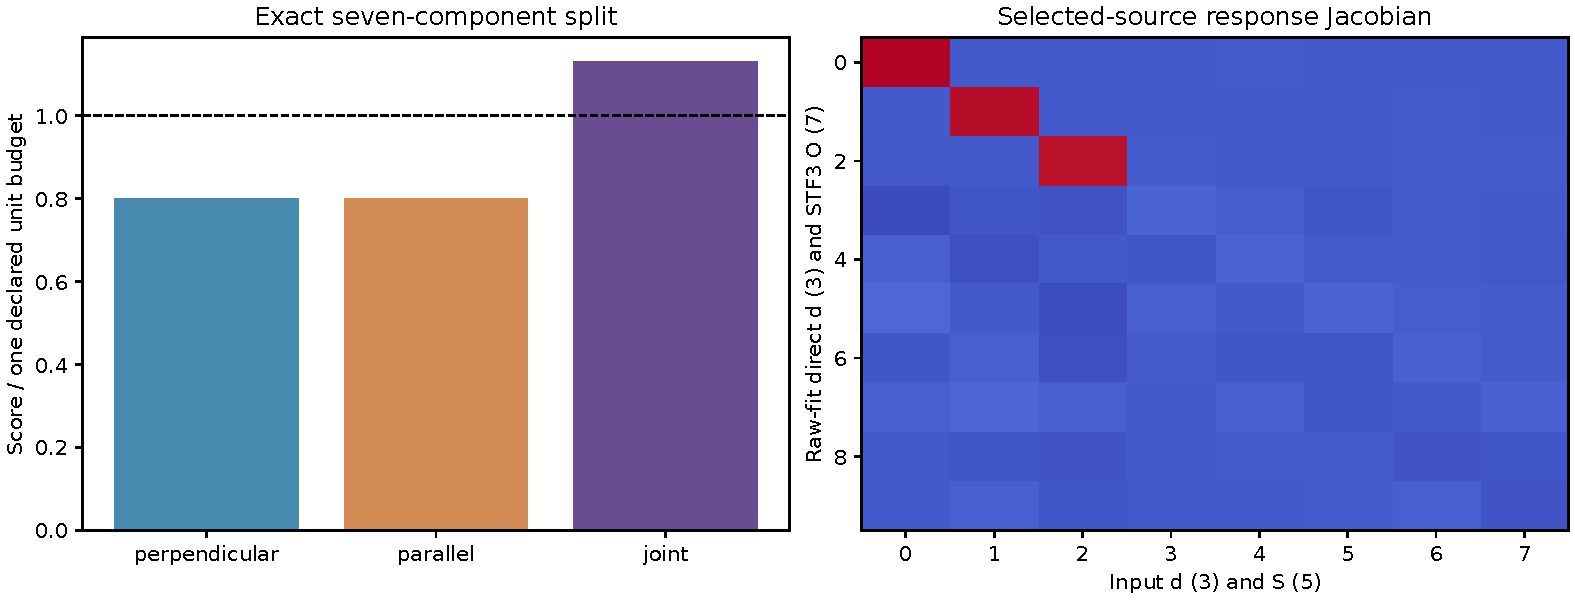
\includegraphics[width=0.94\linewidth]{r36_optical/JOINT_RESPONSE.pdf}
\caption{A shared optical residual budget and a finite selected-source response. Left: the two orthogonal residual components each have size 0.8 of one declared unit budget; their combined norm exceeds that budget. Right: the saved 10-by-8 local Jacobian maps three dimensionless dipole and five dimensionless shear coordinates to three fitted direct-dipole coordinates and seven magnitude-octupole coordinates. Both panels are deterministic mathematical controls. The sampled response is not identified with a physical catalogue dipole.}
\end{figure}

\hypertarget{sampling-covariance-and-finite-distance}{%
\subsection{Sampling, covariance and finite
distance}\label{sampling-covariance-and-finite-distance}}

Before assigning a physical meaning to fitted harmonics, retain the map
from source magnitudes. Let \(T_a^{(2)}\) and \(T_b^{(3)}\) be
Frobenius-orthonormal STF bases. For directions \(n_i\) and positive
weights \(w_i\), use the full-rank 16-column design

\begin{equation}
X_i=(1,n_i^T,T_a^{(2)}:n_in_i,T_b^{(3)}:n_in_in_i),\qquad
 K=J(X^TWX)^{-1}X^TW,\quad W=\operatorname{diag}(w_i).\tag{A6}
\end{equation}

The selector \(J\) multiplies the three fitted magnitude-dipole
coordinates by \(-1/\kappa\) and retains all seven fitted octupole
coordinates. Thus \(Ky\) is a ten-coordinate fitted summary; its first
three entries need not equal the physical \(d\). For the local source
model \(y_i=-\kappa\ln(1+q_i)\), \(q_i=d\cdot n_i+S:n_in_i\), its
derivative is

\begin{equation}
\frac{\partial(Ky)}{\partial(d,S)}
 =K\operatorname{diag}\!\left(\frac{-\kappa}{1+q_i}\right)
       [\,n_i^T,\ T_a^{(2)}:n_in_i\,].\tag{A7}
\end{equation}

The fixed illustration uses 96 deterministic directions, weights
\(1+0.4n_z\), and an input vector \((0.012,-0.009,0.006)\), with the
retained apparent tensor inserted as a mathematical coefficient. The
rank of its sampled design is 16. The direction index is
\(i=0,\ldots,95\), with \(z_i=1-2(i+1/2)/96\),
\(\phi_i=i\pi(3-\sqrt5)\), and
\(n_i=(\sqrt{1-z_i^2}\cos\phi_i,\sqrt{1-z_i^2}\sin\phi_i,z_i)\). These
directions and coefficients are an illustration, not a CF4 data
selection or a measured acceleration.

The signed coordinate convention in this illustration is fixed by
lexicographic Cartesian unit monomials, STF projection, and successive
Frobenius orthogonalization with positive normalization. The full
rank-two and rank-three basis arrays accompany the numerical supplement.
This rank-two coordinate ordering differs from the five-coordinate
display in the main text; the common object is the Cartesian tensor
\(S\), not an untransformed coordinate list.

\begin{table}[htbp]
\centering\small
\caption{Complete signed response of the declared 96-direction mathematical
illustration. The seven octupole entries use the explicit STF basis in
the numerical supplement; neither the fitted direct vector nor this
octupole is a measured CF4 physical quantity.}\label{tab:opticalsigned}
\begin{tabular}{lll}
\hline
Fitted coordinate & Signed value & Unit \\
\hline
$d_x$ & +0.012074086313833 & dimensionless \\
$d_y$ & -0.00903120168213684 & dimensionless \\
$d_z$ & +0.00591810638421224 & dimensionless \\
$O_1$ & -0.000548756550802814 & mag \\
$O_2$ & +0.00040268605514402 & mag \\
$O_3$ & +0.000221664713143214 & mag \\
$O_4$ & -0.000393290392446293 & mag \\
$O_5$ & -4.62789847900094e-06 & mag \\
$O_6$ & +9.87390973288633e-06 & mag \\
$O_7$ & -0.000171094484684956 & mag \\
\hline
\end{tabular}
\end{table}

For a supplied full source covariance \(C_y\), the fitted covariance is
\(C_{10}=KC_yK^T\). At fixed \(\widehat S\), its contribution to the
residual covariance is

\begin{equation}
C_r=A C_{10} A^T,\qquad
 A=[-\kappa L_{\widehat S}\quad I_7].\tag{A8}
\end{equation}

The off-diagonal direct-dipole--octupole blocks contribute to this
expression. The illustration stipulates
\(C_y=10^{-8}(I+0.2uu^T)\,{\rm mag}^2\), where the 96 components of
\(u\) are equally spaced from \(-1\) to \(1\). Its
direct-dipole--octupole cross-block Frobenius norm is
\(1.7820478375045505\times10^{-12}\) in dimensionless-dipole times
magnitude units, and
\(\operatorname{tr}C_r=1.317508814238013\times10^{-8}\,{\rm mag}^2\).
The complete 10-by-10 covariance, 7-by-7 residual covariance and 10-by-8
response derivative are retained, with their coordinate order and units.
This is a source-covariance illustration at fixed \(S\), not a supplied
empirical CF4 covariance, not an uncertain-\(S\) covariance calculation,
and not a confidence region. A confidence threshold would additionally
require a sampling law and its calibration. No unknown empirical
cross-block is filled with zero.

Finite distance requires a separate contribution even when the angular
expansion is controlled. If

\begin{equation}
d_L=\frac{cz}{H(1+q)}[1+z a_1(n)+O(z^2)],\tag{A9}
\end{equation}

then the magnitude correction is \(\kappa z a_1(n)+O(z^2)\), generally
first order in redshift. The saved source-level control uses
\(a_1(n)=T_1^{(3)}:nnn\) and passes \(\kappa\ln[1+za_1(n)]\) through the
same fitted octupole operator. At \(z=(0.02,0.01,0.005)\), its octupole
norms are
\((0.04342971604250298,0.021714693414132947,0.010857342173346137)\) mag.
The successive ratios \(2.0000151608973153\) and \(2.0000008351436778\)
illustrate the leading linear order. These values do not determine a
physical \(B_z\) for a survey; that bound needs a controlled
finite-distance coefficient and the actual estimator and depth weights.

\begin{figure}[htbp]
\centering
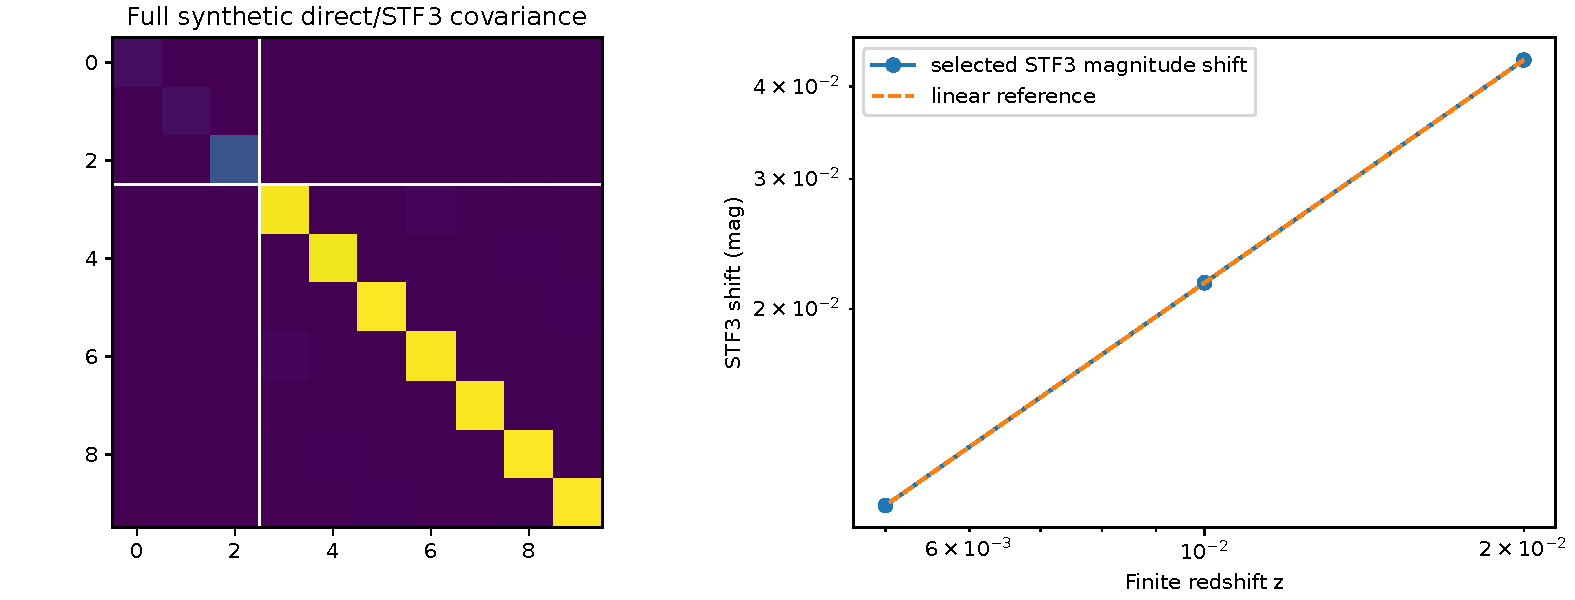
\includegraphics[width=0.94\linewidth]{r36_optical/SOURCE_AND_FINITE_Z.pdf}
\caption{Declared source covariance and a finite-redshift response control. Left: all entries of the synthetic ten-coordinate covariance, ordered as three fitted dimensionless direct-dipole coordinates followed by seven magnitude-octupole coordinates. Entry units follow the corresponding pair of coordinates; the white lines mark the shared-source cross-blocks. The full numerical matrix accompanies the text. Right: the same selected octupole operator applied to a declared relative-distance perturbation, compared with a linear-redshift reference. Neither panel supplies an empirical CF4 joint law or a physical finite-distance error radius.}
\end{figure}

Observer motion also changes the target. The same-congruence coefficient
\(d=-A/(cH)\) is not interchangeable with a peculiar-velocity dipole.
For the dust moving-observer construction, the first-order relation is
\(d_{\rm boost}=-2(I+S)\beta+O(\|\beta\|^2)\), with \(\beta=v/c\); its
inverse requires invertibility of \(I+S\) and control of the omitted
order. At a fixed ray, the Doppler factor \(\Gamma>0\) gives
\(1+\widetilde z=(1+z)/\Gamma\), \(\widetilde d_L=d_L/\Gamma\), and a
shifted vertex \(\widetilde z_o=\Gamma^{-1}-1\). The corrected distance
\(d_L^*=d_L/(1+z)^2\) obeys \(\widetilde d_L^*=\Gamma d_L^*\), so the
vertex derivative transforms as
\(d\widetilde z/d\widetilde d_L^*=\Gamma^{-2}dz/dd_L^*\)
\cite{Maartens2024}. The uncorrected-distance artefact
\(2\operatorname{STF}(\beta\otimes S)\) is distinct from the nonlinear
magnitude octupole \(\kappa L_Sd\). Neither relation turns a raw
catalogue harmonic into a measured acceleration or observer velocity.

\hypertarget{closed-sets-and-numerical-certificates}{%
\subsection{Closed sets and numerical
certificates}\label{closed-sets-and-numerical-certificates}}

The numerical compatibility calculation keeps the two original dipole
balls closed. Finite binary64 coordinates and radii are treated as exact
rational inputs for squared-ball membership and emptiness. Zero-radius
balls and external tangency are handled before optimization. A rounded
tangent point is accepted only if it satisfies both original predicates.
Failure to represent or verify a feasible witness returns numerical
uncertainty, not physical exclusion or an enlarged radius.

An optimizer supplies a candidate, not a compatibility certificate. A
verified feasible candidate supplies a primal residual bound. A lower
bound follows from the seven-component support inequality: for
\(\|u\|\leq1\),

\begin{equation}
r_*\geq u^T\widehat O-h_{\mathcal D}(K_S^Tu),\qquad K_S=\kappa L_{\widehat S},\tag{A10}
\end{equation}

where the support function obeys

\begin{equation}
h_{\mathcal D}(v)\leq
 \min\{v^Td_{\rm obs}+r_d\|v\|,D_{\max}\|v\|\}.\tag{A11}
\end{equation}

If the amplitude ball is omitted, only the first expression is used.
This support bound need not be sharp. The implementation uses candidate
residual and observation directions and incorporates its declared
response-roundoff envelopes. It exports a lower endpoint rounded
downward and an upper endpoint rounded upward. The positive-budget score
is the upward-rounded quotient of the exported upper endpoint and \(B\);
it is an upper bound, not a claim to have computed the exact minimizing
score.

For a general nondegenerate case, the implemented decisions compare the
upper endpoint before display rounding with \(B+\delta_{\rm loc}\), or
the lower endpoint with \(B+\delta_{\rm glob}\). With binary64 machine
epsilon \(\varepsilon_{\rm mach}\), the cancellation allowance is
\(\delta_{\rm loc}=64\varepsilon_{\rm mach}\max(\|\widehat O\|,\|K_Sd_w\|)\)
only when both terms are nonzero and the witness residual is at most
half the larger norm; otherwise it is zero. The conservative rejection
allowance is
\(\delta_{\rm glob}=64\varepsilon_{\rm mach}\max(\|\widehat O\|,\|K_S\|_F D_{\rm cap})\),
where \(D_{\rm cap}\) is the upward-enclosed triangle cap
\(\|d_{\rm obs}\|+r_d\), restricted by \(D_{\max}\) when supplied. These
are numerical response allowances, separate from the physical radii. A
positive cancellation allowance is explicitly recorded, and an accepted
case must not be advertised as a strict zero-allowance residual
certificate unless its exported upper bound also lies below \(B\). A
straddling interval remains numerical uncertainty.

For a singleton set or zero response, the finite-response residual
square is compared with \(B^2\) using exact rational arithmetic,
including equality. A nonzero-response exclusion too close to the
declared global response allowance is still returned as numerical
uncertainty. Underflow of a displayed square does not set a nonzero
residual to zero. The complete certificates retain the witness, endpoint
bounds, response envelope, cancellation allowance and display status.

\begin{table}[htbp]
\centering\small
\caption{Saved finite-response controls. Endpoints bound the profiled residual or
the exact fixed objective under the stated numerical response
conventions; they are not uncertainty intervals for physical
cosmological parameters. Empty-set decisions precede residual
comparison. All radii are stipulated. Full witnesses and all diagnostic
fields accompany the numerical supplement.}\label{tab:opticalcertificates}
\resizebox{\linewidth}{!}{\begin{tabular}{lllll}
\hline
Case & Lower & Upper & $B$ & Result \\
\hline
Shared unit budget & 1.1313708498984756 & 1.1313708498984758 & 1.0 & Incompatible \\
Zero response, zero budget & 0.0 & 0.0 & 0.0 & Compatible \\
Narrow feasible ball & 0.0 & 5.176664520037313e-19 & 5.606717652542515e-10 & Compatible \\
Excluded physical boundary & 2.0184131778458593e-15 & 2.0184235050681796e-15 & 1.0092091825422658e-15 & Incompatible \\
Tangent singleton & 0.0002803358826268454 & 0.00028033588262684546 & 0.001 & Compatible \\
One-spacing interior overlap & 0.00028033588262683885 & 0.00028033588262685186 & 0.001 & Compatible \\
Zero response, fixed sqrt(3) norm & 1.7320508075688772 & 1.7320508075688774 & 2.0 & Compatible \\
Empty direct singleton & --- & --- & --- & Empty \\
Adjacent exterior empty set & --- & --- & --- & Empty \\
\hline
\end{tabular}}
\end{table}

The near-tangent examples make the closed-set convention concrete. Set
both radii to \(1/8\). A center \((1/4,0,0)\) has the representable
unique intersection \((1/8,0,0)\). For the adjacent binary64 center
below \(1/4\), a feasible saved witness is
\((0.12499999999999999,0,0)\); with
\(S=\operatorname{diag}(0.001,-0.001,0)\), zero observed octupole and
\(B=0.001\), its exported upper residual bound is
\(0.00028033588262685186<B\). The adjacent center above \(1/4\) gives an
exactly empty intersection. A direct singleton at \((1/8,10^{-60},0)\)
lies outside the physical ball of radius \(1/8\): the second component
gives a strictly positive exact squared excess, even when a rounded norm
hides it. The decimal \(10^{-60}\) here denotes its supplied binary64
value, whose square is near \(10^{-120}\), not exactly that decimal
rational. Zero and nonzero shear controls also preserve a residual of
\(10^{-200}\) against a zero budget. These examples test witness
availability and range handling; they do not prove that every feasible
real intersection has a representable witness or that every numerical
optimization is decisive.

The physical output remains a conditional response-compatible set. The
apparent tensor, source-covariance illustration and numerical controls
do not supply an empirical joint direct-dipole--octupole law, the
missing finite-distance and selection bounds, or a common physical
source/observer transfer. Vorticity, curvature, energy, absolute
expansion and history remain unresolved as described in the main text.
Full signed coordinates and shared dependence must be retained before
any later scalar summary or physical attribution.
